%%%%%%%%%%%%%%%%%%%%%%%%%%%%%%%%%%%%%%%%%%%%%%%%%%%%%%%%%%%%%%%%%%%%%%%%%%%%%%%%
% TUM-Vorlage: Plakat A1 Querformat
%%%%%%%%%%%%%%%%%%%%%%%%%%%%%%%%%%%%%%%%%%%%%%%%%%%%%%%%%%%%%%%%%%%%%%%%%%%%%%%%
%
% Rechteinhaber:
%     Technische Universität München
%     https://www.tum.de
% 
% Gestaltung:
%     ediundsepp Gestaltungsgesellschaft, München
%     http://www.ediundsepp.de
% 
% Technische Umsetzung:
%     eWorks GmbH, Frankfurt am Main
%     http://www.eworks.de
%
%%%%%%%%%%%%%%%%%%%%%%%%%%%%%%%%%%%%%%%%%%%%%%%%%%%%%%%%%%%%%%%%%%%%%%%%%%%%%%%%

%%%%%%%%%%%%%%%%%%%%%%%%%%%%%%%%%%%%%%%%%%%%%%%%%%%%%%%%%%%%%%%%%%%%%%%%%%%%%%%%
\documentclass[a1, plainsections, landscape]{sciposter}
\newcommand{\PlakatFormat}{A1 quer}

\usepackage[utf8]{inputenc} % Textkodierung: UTF-8
\usepackage[T1]{fontenc} % Zeichensatzkodierung

\usepackage[ngerman]{babel} % Deutsche Lokalisierung
\usepackage{graphicx} % Grafiken
\usepackage{calc} % Berechnungen

% Silbentrennung:
\usepackage{hyphenat}
%\tolerance 2414
%\hbadness 2414
%\emergencystretch 1.5em
%\hfuzz 0.3pt
%\widowpenalty=10000     % Hurenkinder
%\clubpenalty=10000      % Schusterjungen
%\vfuzz \hfuzz

% Euro-Symbol:
\usepackage[gen]{eurosym}
\DeclareUnicodeCharacter{20AC}{\euro{}}

% Schriftart Helvetica:
\usepackage[scaled]{helvet}
\renewcommand{\familydefault}{\sfdefault}

\usepackage{mathptmx} % skalierbare Formelschriften

\usepackage{multicol} % mehrspaltiger Text
%\usepackage{showframe} % Seitenbegrenzungen anzeigen
\usepackage{lipsum} % Blindtext

\newcommand{\PlakatFusszeileSpaltenzahl}{}

\makeatletter
\newcommand{\@minipagerestore}{\setlength{\parskip}{\medskipamount}}%
\makeatother

% Längen:
\newlength{\PlakatSeiteHoehe}
\newlength{\PlakatSeiteRand}
\newlength{\PlakatKopfzeileHoehe}
\newlength{\PlakatKopfzeileAbstand}
\newlength{\PlakatFusszeileHoehe}
\newlength{\PlakatUniversitaetLogoBreite}
\newlength{\PlakatFakultaetLogoBreite}
\newlength{\PlakatPositionLinks}
\newlength{\PlakatKopfzeilePositionUnten}
\newlength{\PlakatFakultaetslogoPositionKorrekturLinks}
\newlength{\PlakatFakultaetslogoPositionKorrekturOben}
\newlength{\PlakatFakultaetslogoAbstandRechts}
\newlength{\PlakatFusszeilePositionUnten}
\newlength{\PlakatFusszeilePositionKorrektur}
\newlength{\PlakatTitelZweiPlatzDanach}
\newlength{\PlakatTitelDreiPlatzDanach}
\newlength{\PlakatUniversitaetslogoPositionKorrekturLinks}
\newlength{\PlakatSpaltenAbstand}
\newlength{\PlakatSchriftNormalGroesse}
\newlength{\PlakatSchriftNormalZeilenabstand}
\newlength{\PlakatAufzaehlungAbstandLinks}

% Einspaltigkeit ist nur für A3 und A4 verfügbar:
\newlength{\PlakatEinspaltigPositionKorrekturOben}
\newlength{\currentbaselineskip}
\newlength{\currentparskip}
\newlength{\currentparindent}

\newenvironment{PlakatEinspaltig}{%
    \setlength{\currentbaselineskip}{\baselineskip}%
    \setlength{\currentparskip}{\parskip}%
    \setlength{\currentparindent}{\parindent}%
    \vspace*{\PlakatEinspaltigPositionKorrekturOben}%
    \begin{minipage}[t][0cm]{\textwidth}% Höhe von 0cm sorgt für das Bleiben auf der gleichen Seite
    \setlength{\baselineskip}{\currentbaselineskip}%
    \setlength{\parskip}{\currentparskip}%
    \setlength{\parindent}{\currentparindent}%
    \raggedright\empty%
}
{%
    \end{minipage}%
}

\newsavebox{\TempBox}

\newcommand{\PlakatBildBeschnitt}{0cm 0cm 0cm 0cm}

\newcommand{\PlakatBild}[3][0cm 0cm 0cm 0cm]{%
    \vspace{-\baselineskip}%
    \begin{figure}%
        \includegraphics[width=\textwidth, trim=#1, clip=true]{#2}%
        \PlakatBildUnterschrift{#3}%
    \end{figure}%
    \vspace{-\baselineskip}%
}

\newcommand{\PlakatBildGanzseitig}[3][0cm 0cm 0cm 0cm]{%
    \begin{minipage}[t][0cm]{\paperwidth-\PlakatSeiteRand-\PlakatSeiteRand}%
    \PlakatBild[#1]{#2}{#3}%
    \end{minipage}
}

% Für Beischreibung:
\newlength{\PlakatBeschreibungBeispielbildBeschnitt}
\setlength{\PlakatBeschreibungBeispielbildBeschnitt}{0cm}
\newcommand{\PlakatBeschreibungBeispielbild}{true}
\newcommand{\PlakatBeschreibungKopfzeileUndAbsender}{true}
\newcommand{\PlakatBeschreibungDruck}{true}
\newcommand{\PlakatBeschreibungKurz}{false}
\newcommand{\TRUE}{true}

\setlength{\PlakatFusszeilePositionUnten}{47.5mm}
\renewcommand{\PlakatFusszeileSpaltenzahl}{6}

\setlength{\PlakatSeiteRand}{35mm}
\setlength{\PlakatKopfzeileHoehe}{4cm}
\setlength{\PlakatKopfzeileAbstand}{26mm}
\setlength{\PlakatKopfzeilePositionUnten}{25.5mm}
\setlength{\PlakatUniversitaetLogoBreite}{66.5mm}
\setlength{\PlakatFakultaetLogoBreite}{42mm}
\setlength{\PlakatPositionLinks}{-1cm}
\setlength{\PlakatFakultaetslogoPositionKorrekturLinks}{28.5mm}
\setlength{\PlakatFakultaetslogoPositionKorrekturOben}{2.5mm}
\setlength{\PlakatFakultaetslogoAbstandRechts}{12mm}
\setlength{\PlakatUniversitaetslogoPositionKorrekturLinks}{-9.5mm}
\setlength{\PlakatSpaltenAbstand}{14mm}
\setlength{\PlakatSchriftNormalGroesse}{22pt}
\setlength{\PlakatSchriftNormalZeilenabstand}{27pt}
\setlength{\PlakatFusszeileHoehe}{28mm}
\setlength{\PlakatAufzaehlungAbstandLinks}{0.7em}

\newcommand{\PlakatTitelSchriftgroesse}{\fontsize{67}{80}\selectfont}

\newcommand{\PlakatTitelEins}[1]{{\PlakatTitelSchriftgroesse #1}\\[38pt]}
\newcommand{\PlakatTitelZwei}[1]{{\fontsize{49}{53}\selectfont #1}\\[19pt]}
\newcommand{\PlakatTitelDrei}[1]{{\fontsize{39}{10}\selectfont #1}\\[68pt]}

\newcommand{\PlakatKopfzeileSchriftgroesse}{\fontsize{30}{39}}
\newcommand{\PlakatFusszeileSchrift}{\fontsize{11}{13.2}\selectfont}
\newcommand{\PlakatBildUnterschrift}[1]{{\\[-3mm]\fontsize{14}{18}\selectfont{}#1}}


\setlength{\PlakatSeiteHoehe}{42.9cm} % !!! NICHT ENTFERNEN !!!
%%%%%%%%%%%%%%%%%%%%%%%%%%%%%%%%%%%%%%%%%%%%%%%%%%%%%%%%%%%%%%%%%%%%%%%%%%%%%%%%
% TUM-Vorlage: Personenspezifische Informationen
%%%%%%%%%%%%%%%%%%%%%%%%%%%%%%%%%%%%%%%%%%%%%%%%%%%%%%%%%%%%%%%%%%%%%%%%%%%%%%%%
%
% Rechteinhaber:
%     Technische Universität München
%     https://www.tum.de
% 
% Gestaltung:
%     ediundsepp Gestaltungsgesellschaft, München
%     http://www.ediundsepp.de
% 
% Technische Umsetzung:
%     eWorks GmbH, Frankfurt am Main
%     http://www.eworks.de
%
%%%%%%%%%%%%%%%%%%%%%%%%%%%%%%%%%%%%%%%%%%%%%%%%%%%%%%%%%%%%%%%%%%%%%%%%%%%%%%%%

% Für die Person anpassen:

\newcommand{\PersonTitel}{G10}
\newcommand{\PersonVorname}{Erika}
\newcommand{\PersonNachname}{Mustermann}
\newcommand{\PersonStadt}{@Ort@}
\newcommand{\PersonAdresse}{%
    @Adresse@\\%
    @Plz@~\PersonStadt%
}
\newcommand{\PersonTelefon}{@Telefon@}
\newcommand{\PersonFax}{@Fax@}
\newcommand{\PersonEmail}{@E-Mail@}
\newcommand{\PersonWebseite}{@Web@}

\newcommand{\FakultaetAnsprechpartner}{@Ansprechpartner@}
% Fakultät:
\newcommand{\FakultaetName}{Fakultät für Elektrotechnik und Informationstechnik}
\newcommand{\LehrstuhlName}{Lehrstuhl für Datenverarbeitung}

\newcommand{\EinstellungBankName}{Bayerische Landesbank}
\newcommand{\EinstellungBankIBAN}{DE10700500000000024866}
\newcommand{\EinstellungBankBIC}{BYLADEMM}
\newcommand{\EinstellungSteuernummer}{143/241/80037}
\newcommand{\EinstellungUmsatzsteuerIdentifikationsnummer}{DE811193231}

\hyphenation{} % eigene Silbentrennung                    % !!! DATEI ANPASSEN !!!
%%%%%%%%%%%%%%%%%%%%%%%%%%%%%%%%%%%%%%%%%%%%%%%%%%%%%%%%%%%%%%%%%%%%%%%%%%%%%%%%


\newcommand{\PlakatTitel}{CLSM - Convolutional Latent Semantic Model}


%%%%%%%%%%%%%%%%%%%%%%%%%%%%%%%%%%%%%%%%%%%%%%%%%%%%%%%%%%%%%%%%%%%%%%%%%%%%%%%%
%%%%%%%%%%%%%%%%%%%%%%%%%%%%%%%%%%%%%%%%%%%%%%%%%%%%%%%%%%%%%%%%%%%%%%%%%%%%%%%%
% EINSTELLUNGEN
%%%%%%%%%%%%%%%%%%%%%%%%%%%%%%%%%%%%%%%%%%%%%%%%%%%%%%%%%%%%%%%%%%%%%%%%%%%%%%%%

% Allgemein:
\newcommand{\AllgemeinGestalter}{ediundsepp Gestaltungsgesellschaft}
\newcommand{\AllgemeinErsteller}{eWorks GmbH}

% Universität:
\newcommand{\UniversitaetName}{Technische Universität München}
\newcommand{\UniversitaetAbkuerzung}{TUM}
\newcommand{\UniversitaetWebseite}{www.tum.de}
\newcommand{\UniversitaetLogoBreite}{19mm}
\newcommand{\UniversitaetLogoHoehe}{1cm}

\newcommand{\UniversitaetAdresse}{%
    Arcisstraße~21\\%
    80333~München%
}


% Seitenränder:
\newcommand{\SeitenrandOben}{20mm}
\newcommand{\SeitenrandRechts}{20mm}
\newcommand{\SeitenrandLinks}{25mm}
\newcommand{\SeitenrandUnten}{10mm}

% Falzmarken:
\newcommand{\FalzmarkeOben}{87mm}
\newcommand{\FalzmarkeMitte}{148.5mm}
\newcommand{\FalzmarkeUnten}{192mm}
\newcommand{\FalzmarkeBreite}{2mm}
\newcommand{\FalzmarkeDicke}{0.3pt}
\newcommand{\FalzmarkePositionLinks}{7mm}


% Adressfeld:
\newcommand{\AdressfeldHoehe}{45mm}
\newcommand{\AdressfeldBreite}{85mm}
\newcommand{\AdressfeldAbsenderSchriftgroesse}{7.5pt}
\newcommand{\AdressfeldEmpfaengerSchriftgroesse}{11pt}
\newcommand{\AdressfeldEmpfaengerZeilenabstand}{15pt}

% Text:
\newcommand{\TextOben}{77.5mm}
\newcommand{\TextSchriftgroesse}{11pt}
\newcommand{\TextZeilenabstand}{15pt}

% Fusszeile:
\newcommand{\FusszeilePositionOben}{271mm}
\newcommand{\FusszeileBreite}{165mm}
\newcommand{\FusszeileHoehe}{16.5mm}
\newcommand{\FusszeileZwischenabstand}{2mm}
\newcommand{\FusszeileBreiteGross}{44mm}
\newcommand{\FusszeileBreiteKlein}{35.5mm}
\newcommand{\FusszeileSeitennummerAbstand}{7.7mm}
\newcommand{\FusszeileSchriftgroesse}{7.5pt}
\newcommand{\FusszeileZeilenabstand}{8pt}


%%%%%%%%%%%%%%%%%%%%%%%%%%%%%%%%%%%%%%%%%%%%%%%%%%%%%%%%%%%%%%%%%%%%%%%%%%%%%%%%
% DOKUMENT
%%%%%%%%%%%%%%%%%%%%%%%%%%%%%%%%%%%%%%%%%%%%%%%%%%%%%%%%%%%%%%%%%%%%%%%%%%%%%%%%

\usepackage[a4paper,
    top=\SeitenrandOben,
    bottom=\SeitenrandUnten,
    inner=\SeitenrandLinks,
    outer=\SeitenrandRechts,
    foot=\FusszeileHoehe - 1mm,
    head=0cm,
    includefoot
]{geometry}

\textblockorigin{\SeitenrandLinks}{\SeitenrandOben} % Ursprung für Positionierung

% PDF-Einstellungen:
\usepackage[pdftex]{hyperref}
\hypersetup{
    hidelinks,
    pdfauthor={\PersonVorname{} \PersonNachname},
    pdftitle={\Betreff},
    pdfproducer={\AllgemeinErsteller},
    pdfcreator={\AllgemeinGestalter}
}

\renewcommand*{\raggedsignature}{\raggedright}

\makeatletter
    \@setplength{bfoldmarklength}{\FalzmarkeBreite}
    \@setplength{bfoldmarkvpos}{\FalzmarkeUnten}
    \@setplength{firstfoothpos}{\SeitenrandLinks - 2pt}
    \@setplength{firstfootvpos}{\FusszeilePositionOben}
    \@setplength{firstfootwidth}{\FusszeileBreite}
    \@setplength{foldmarkhpos}{\FalzmarkePositionLinks}
    \@setplength{foldmarkthickness}{\FalzmarkeDicke}
    \@setplength{mfoldmarklength}{\FalzmarkeBreite}
    \@setplength{mfoldmarkvpos}{\FalzmarkeMitte}

    \@setplength{refaftervskip}{\TextZeilenabstand}
    \@setplength{refvpos}{\TextOben}
    \@setplength{sigbeforevskip}{\baselineskip}
    \@setplength{sigindent}{0mm}
    \@setplength{subjectaftervskip}{\baselineskip + \baselineskip + 1pt}

    \@setplength{tfoldmarklength}{\FalzmarkeBreite}
    \@setplength{tfoldmarkvpos}{\FalzmarkeOben}
\makeatother

\KOMAoptions{
    fontsize=\TextSchriftgroesse,
    foldmarks=BMpTv,
    firsthead=false,
    backaddress=no,
    addrfield=no,
    fromalign=false
}

\setkomavar{fromname}{\UniversitaetName}
\setkomavar{fromaddress}{\PersonAdresse}
\addtokomafont{backaddress}{\fontsize{\AdressfeldAbsenderSchriftgroesse}{\AdressfeldAbsenderSchriftgroesse}\selectfont}
\addtokomafont{toaddress}{\fontsize{\AdressfeldEmpfaengerSchriftgroesse}{\AdressfeldEmpfaengerZeilenabstand}\selectfont}

\newcommand{\RuecksendeadresseTrenner}{~| \ignorespaces}

\AtBeginLetter{%
    % Logo:
    \begin{textblock*}{\UniversitaetLogoBreite}[1,0](\textwidth, 0cm)%
        \raggedleft%
        
\includegraphics{./Ressourcen/_Bilder/Universitaet_Logo_RGB.pdf}%
    \end{textblock*}%
    \setlength{\baselineskip}{\TextZeilenabstand}%
    \setlength{\parindent}{0mm} % keine Einrückung am Absatzanfang
    \setlength{\parskip}{\baselineskip} % einzeiliger Abstand nach Absätzen
    % Empfängerfenster:
    \begin{textblock*}{\AdressfeldBreite}[0,0](0cm, 15mm)%
        \raggedbottom\raggedright
        \begin{spacing}{.85}%
        {
            \usekomafont{backaddress}%
            \let\\\RuecksendeadresseTrenner% Umdefinieren von "\\" zu "~| "
            \Absender%
        } \\
        \end{spacing}
        \vspace*{5.5pt}
        \usekomafont{toaddress}%
        \EmpfaengerAdresse
    \end{textblock*}
}

\KOMAoptions{refline=dateleft}
\setkomavar{date}{\Datum}
\setkomavar{place}{\PersonStadt}
\setkomafont{subject}{\bfseries}
\setkomavar{subject}{\Betreff}
\setkomavar{signature}{\PersonVorname~\PersonNachname}

%\setkomavar*{enclseparator}{Anlage\vspace{-3em}}

\renewcommand*{\closing}[1]{#1\vspace*{3\baselineskip}\newline\usekomavar{signature}\newline}
\setkomavar{enclseparator}[Anlage]{~}
\renewcommand{\encl}[1]{\newline{}Anlage~#1}

\KOMAoptions{firstfoot=true}
\setkomafont{pagefoot}{\sffamily\fontsize{7.5pt}{8pt}\selectfont}
\renewcommand{\pagemark}{%
\begin{textblock*}{3em}[1,1](\paperwidth - \SeitenrandLinks - \SeitenrandRechts + \FusszeileSeitennummerAbstand + 3mm, \paperheight - \SeitenrandOben - \SeitenrandUnten)%
    \raggedleft\hfill\usekomafont{pagefoot}\thepage\,/\,\pageref*{LastPage}%
\end{textblock*}%
}

\setkomavar{firstfoot}{
    \TabPositions{2em}%
    \begin{minipage}[t][\FusszeileHoehe][t]{\FusszeileBreiteGross}%
        \usekomafont{pagefoot}%
        \textbf{\UniversitaetName}%
        \newline%
        \FakultaetName%
        \newline%
        \LehrstuhlName%
    \end{minipage}%
    \hspace*{\FusszeileZwischenabstand}%
    \begin{minipage}[t][\FusszeileHoehe][t]{\FusszeileBreiteGross}%
        \raggedright\usekomafont{pagefoot}%
        \textbf{\FakultaetAnsprechpartner}\newline%
        \PersonAdresse%
    \end{minipage}%
    \hspace*{\FusszeileZwischenabstand}%
    \begin{minipage}[t][\FusszeileHoehe][t]{\FusszeileBreiteKlein}%
        \raggedright\usekomafont{pagefoot}%
        Tel.\tab{\PersonTelefon}%
        \def\temp{\PersonFax}\ifx\temp\empty%
        \else%
          \newline Fax\tab{\PersonFax}%
        \fi%
        \newline\newline%
        \PersonEmail\newline%
        \href{http://\PersonWebseite}{\PersonWebseite}\newline%
        \href{http://\UniversitaetWebseite}{\UniversitaetWebseite}%
    \end{minipage}%
    \hspace*{\FusszeileZwischenabstand}%
    \begin{minipage}[t][\FusszeileHoehe][t]{\FusszeileBreiteKlein}%
        \raggedright\usekomafont{pagefoot}%
        \EinstellungBankName\newline%
        IBAN-Nr.: \EinstellungBankIBAN\newline%
        BIC: \EinstellungBankBIC\newline%
        Steuer-Nr.: \EinstellungSteuernummer\newline%
        USt-IdNr.: \EinstellungUmsatzsteuerIdentifikationsnummer\newline%
    \end{minipage}%
    \pagemark%
}

\begin{document}
\raggedright
\begin{letter}{\EmpfaengerAdresse{}}
\opening{\Gruss}

 % !!! NICHT ENTFERNEN !!!
%%%%%%%%%%%%%%%%%%%%%%%%%%%%%%%%%%%%%%%%%%%%%%%%%%%%%%%%%%%%%%%%%%%%%%%%%%%%%%%%



%%%%%%%%%%%%%%%%%%%%%%
%% 3-Spalten-Layout %%
%%%%%%%%%%%%%%%%%%%%%%

\PlakatKopfzeileMitDreizeiler
\PlakatFusszeileLeer

\PlakatTitelEins{\PlakatTitel}
\PlakatTitelZwei{A Latent Semantic Model with Convolutional-Pooling Structure for Information Retrieval}
\PlakatTitelDrei{G10 - Moustafa AboulAtta, Martin Achtner, Ridon Arifi, Daniel Ehrhardt and Lukas Fichtner}

\begin{multicols*}{3}

%\setlength{\PlakatBeschreibungBeispielbildBeschnitt}{50cm} % Anpassen der Größe des Beispielbildes
%\PlakatUeberschrift{Schriftgröße 11 pt}

Dies ist die Vorlage für das Plakat (DIN \PlakatFormat{}) der Technischen
Universität München (TUM). Sie entspricht dem Corporate Design der TUM und ist für das Betriebssystem Windows getestet und mit TeX Live 2015 kompatibel.

Bitte geben Sie Ihren individuellen Text an den vorgesehenen Stellen ein. Nutzerhinweise finden Sie außerdem in der Liesmich.txt.

\ifx\PlakatBeschreibungKopfzeileUndAbsender\TRUE
\PlakatUeberschrift{Kopfzeile und Absender}

Es stehen mehrere Varianten zur Auswahl. Diese finden Sie auf den nächsten Seiten als Beispiel oder unter \href{http://\UniversitaetWebseite/cd}{\UniversitaetWebseite/cd}, welche für die verschiedenen Nutzergruppen vorgesehen sind.

\fi

\PlakatUeberschrift{Text}

Strukturieren Sie Ihr Plakat möglichst klar und beschränken Sie sich auf die wichtigsten Informationen. Entscheiden Sie sich für einen ein- oder mehrspaltigen Aufbau, linksbündig oder im Blocksatz. Und wählen Sie bei wenig Text eine entsprechend größere Schrift.

\PlakatUeberschrift{Bilder}

\ifx\PlakatBeschreibungKurz\TRUE % BEGINN kurze/lange Beschreibung

Auch wenn Sie Bilder integrieren möchten, können Sie innerhalb des vorgegebenen Rahmens variieren:

\begin{itemize}
\item Das Bild ist an die Breite der Textspalte angepasst
\item Das Bild geht über alle Textspalten
\item Das Bild ist seitenfüllend innerhalb des vorgesehenen Textrahmens (mit weißem Rand)
\item Das Bild ist seitenfüllend bis an den Papierrand (randabfallend) an mindestens drei Seiten
\end{itemize}

Bilder sollten immer eine Bildunterschrift tragen, die ggf. Informationen zum Bild und zur Autorenschaft enthält.
Das Bild sollte immer genügend Abstand zum Text haben. Gleiches gilt für Grafiken.

\else

Auch wenn Sie Bilder integrieren möchten, können Sie innerhalb des vorgegebenen Rahmens variieren:

\begin{itemize}
\item Das Bild ist an die Breite der Textspalte angepasst
\item Das Bild geht über alle Textspalten
\item Das Bild ist seitenfüllend innerhalb des vorgesehenen Textrahmens (mit weißem Rand)
\item Das Bild ist seitenfüllend bis an den Papierrand (randabfallend) an mindestens drei Seiten
\end{itemize}

Bilder sollten immer eine Bildunterschrift tragen, die ggf. Informationen zum Bild und zur Autorenschaft enthält. 
Das Bild sollte immer genügend Abstand zum Text haben. Gleiches gilt für Grafiken.

\ifx\PlakatBeschreibungBeispielbild\TRUE
\PlakatBild[0cm \PlakatBeschreibungBeispielbildBeschnitt{} 0cm 0cm]{./Ressourcen/_Bilder/Sternenhimmel.jpg}{Bildunterschrift, Autor etc}
\fi

\ifx\PlakatBeschreibungDruck\TRUE
\PlakatUeberschrift{Druck}

Achten Sie darauf, dass das Dokument in Originalgröße gedruckt wird, also keine Anpassung an die Druckränder bei Ihren Druckereinstellungen aktiviert ist.
Wählen Sie bitte unbedingt weiße Papiere statt Naturpapier mit starker Braun- oder Graufärbung. Denn nur sie entsprechen dem Charakter des Corporate Designs der TUM. Denken Sie daran, dass auch Papierstärke (Dicke) und Haptik einen Einfluss auf das Druckergebnis haben.
\fi

\fi % ENDE kurze/lange Beschreibung

Weitere Informationen zum Corporate Design der TUM finden Sie unter
\href{http://\UniversitaetWebseite/cd}{\UniversitaetWebseite/cd}


\PlakatUeberschrift{Introduction}

\begin{itemize}

\item Modern search engines rely on semantic models for the retrieval of Web documents with search queries.

\item These perform better than simple lexical models by combining words that appear in a similar context into semantic clusters.

\item However existing models do mostly not consider the context of the words which can lead to unwanted results. (e.g. microsoft \textit{office} $\leftrightarrow$ apartment \textit{office})

\item CLSM is taking the context into account and is thus able to achieve a better performance.

\end{itemize}


\PlakatUeberschrift{CLSM Architecture}
The CLSM consists of five layers (c. Figure 1) in the following order:\\
\vspace{20mm}
%\begin{enumerate}
%	\item Word-n-gram layer
%		\begin{itemize}
%			\item Run a contextual sliding window of size n over the input word sequence $\rightarrow$ Separation into word-n-grams
%			\item Add passing words (<s>) at beginning and end of the sequence $\rightarrow$ fragment for each word is of equal length
%		\end{itemize}
	
%	\item Letter-trigram layer
	
%		\begin{itemize}
%			\item Segment the single words into letter-trigrams.
%			\item Represent the word as a count vector f of the trigrams.
			%\begin{equation}
			%f('word') = \begin{array}{c}0\\...\\1\\...\\1\\...\\1\\...\\1\\...\\0\end{array}
			%\end{equation}
%			\item Build word-n-grams for each of the words by putting n count vectors together in a vector $l$ like this:
%				\begin{equation}
%					l_t = [f_{t-d}^T, ..., f_{t}^T, ..., s_{t+d}^T]^T \hspace{20mm} n = 2d + 1,\hspace{5mm} t = 1...T\footnote{\label{foot:1} T: Number of words in the input word sequence}
%				\end{equation}
%		\end{itemize}
	
%	\item Convolutional layer
	
%		\begin{itemize}
%			\item Project $l_t$ to a contextual feature vector $h_t$ through the convolution matrix $W_c$
%				\begin{equation}
%					h_t = tanh(W_c \cdot l_t) \hspace{20mm} t = 1...T
%				\end{equation}
%			\item Here tanh denotes the activation function of the underlying neural network.
%		\end{itemize}
%\vfill
%\columnbreak

%	\item Max-pooling layer
%		\begin{itemize}
%			\item Combine the local feature vectors into one global vector by taking the maximum of each dimension of the vectors. (max pooling)
%				\begin{equation}
%				v(i) = \max\limits_{t=1,...,T}\{h_t(i)\} \hspace{20mm} i = 1, ..., K\footnote{\label{foot:2} K: Dimensionality of the max pooling layer}
%				\end{equation}
%		\end{itemize}
%	\item Semantic layer
%		\begin{itemize}
%			\item Extract the high-level semantic representation through one more non-linear transformation with the semantic projection matrix $W_s$.
%				\begin{equation}
%					y = tanh(W_s \cdot v)
%				\end{equation}
%		\end{itemize}
%\end{enumerate}

% Bild zur Architektur

\PlakatBild[-5mm \PlakatBeschreibungBeispielbildBeschnitt{} -5mm 0cm]{Architektur.png}{\textbf{Figure 1:} The Architecture of CLSM, Shen et al.}



\setlength{\PlakatBeschreibungBeispielbildBeschnitt}{50cm} % Anpassen der Größe des Beispielbildes

\columnbreak

\PlakatUeberschrift{Usage}
\begin{itemize}
	\item Use the CLSM model on the query and the documents
	\item Determine the matching documents via the cosine distance of the resulting vectors
\end{itemize}

\vspace{5mm}
\begin{figure}

	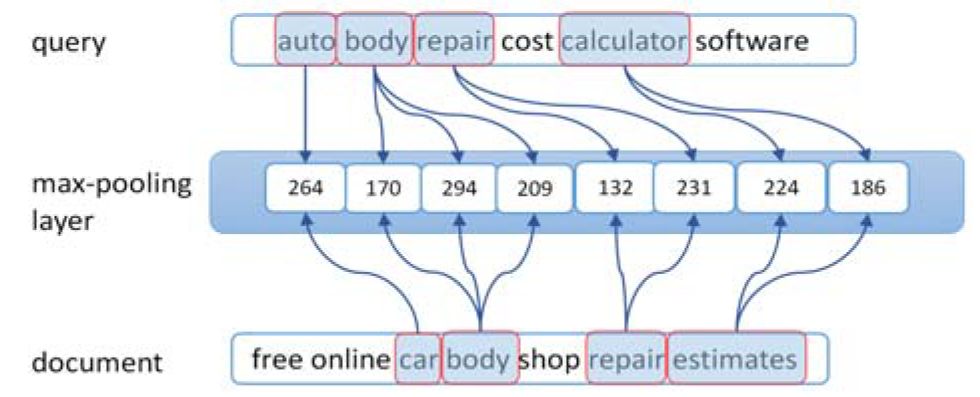
\includegraphics[width = \textwidth]{./SemanticMatching.png}\\
	\PlakatBildUnterschrift{\textbf{Figure 2:} Semantic Matching on Maxpooling Layer, Shen et al.}

\end{figure}


\PlakatUeberschrift{Learning}

\begin{itemize}
	\item Model paramaters are trained to maximize the likelihood P(D+|Q) through the loss function.
\end{itemize}

\vspace{5mm}
\begin{figure}
	
	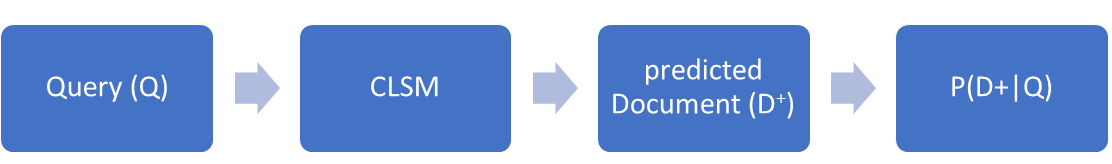
\includegraphics[width = \textwidth]{./learning.png}\\
	\PlakatBildUnterschrift{\textbf{Figure 3:} CLSM learning process}
	
\end{figure}

\columnbreak

\PlakatUeberschrift{Experiments and Results}

%\begin{figure}
%	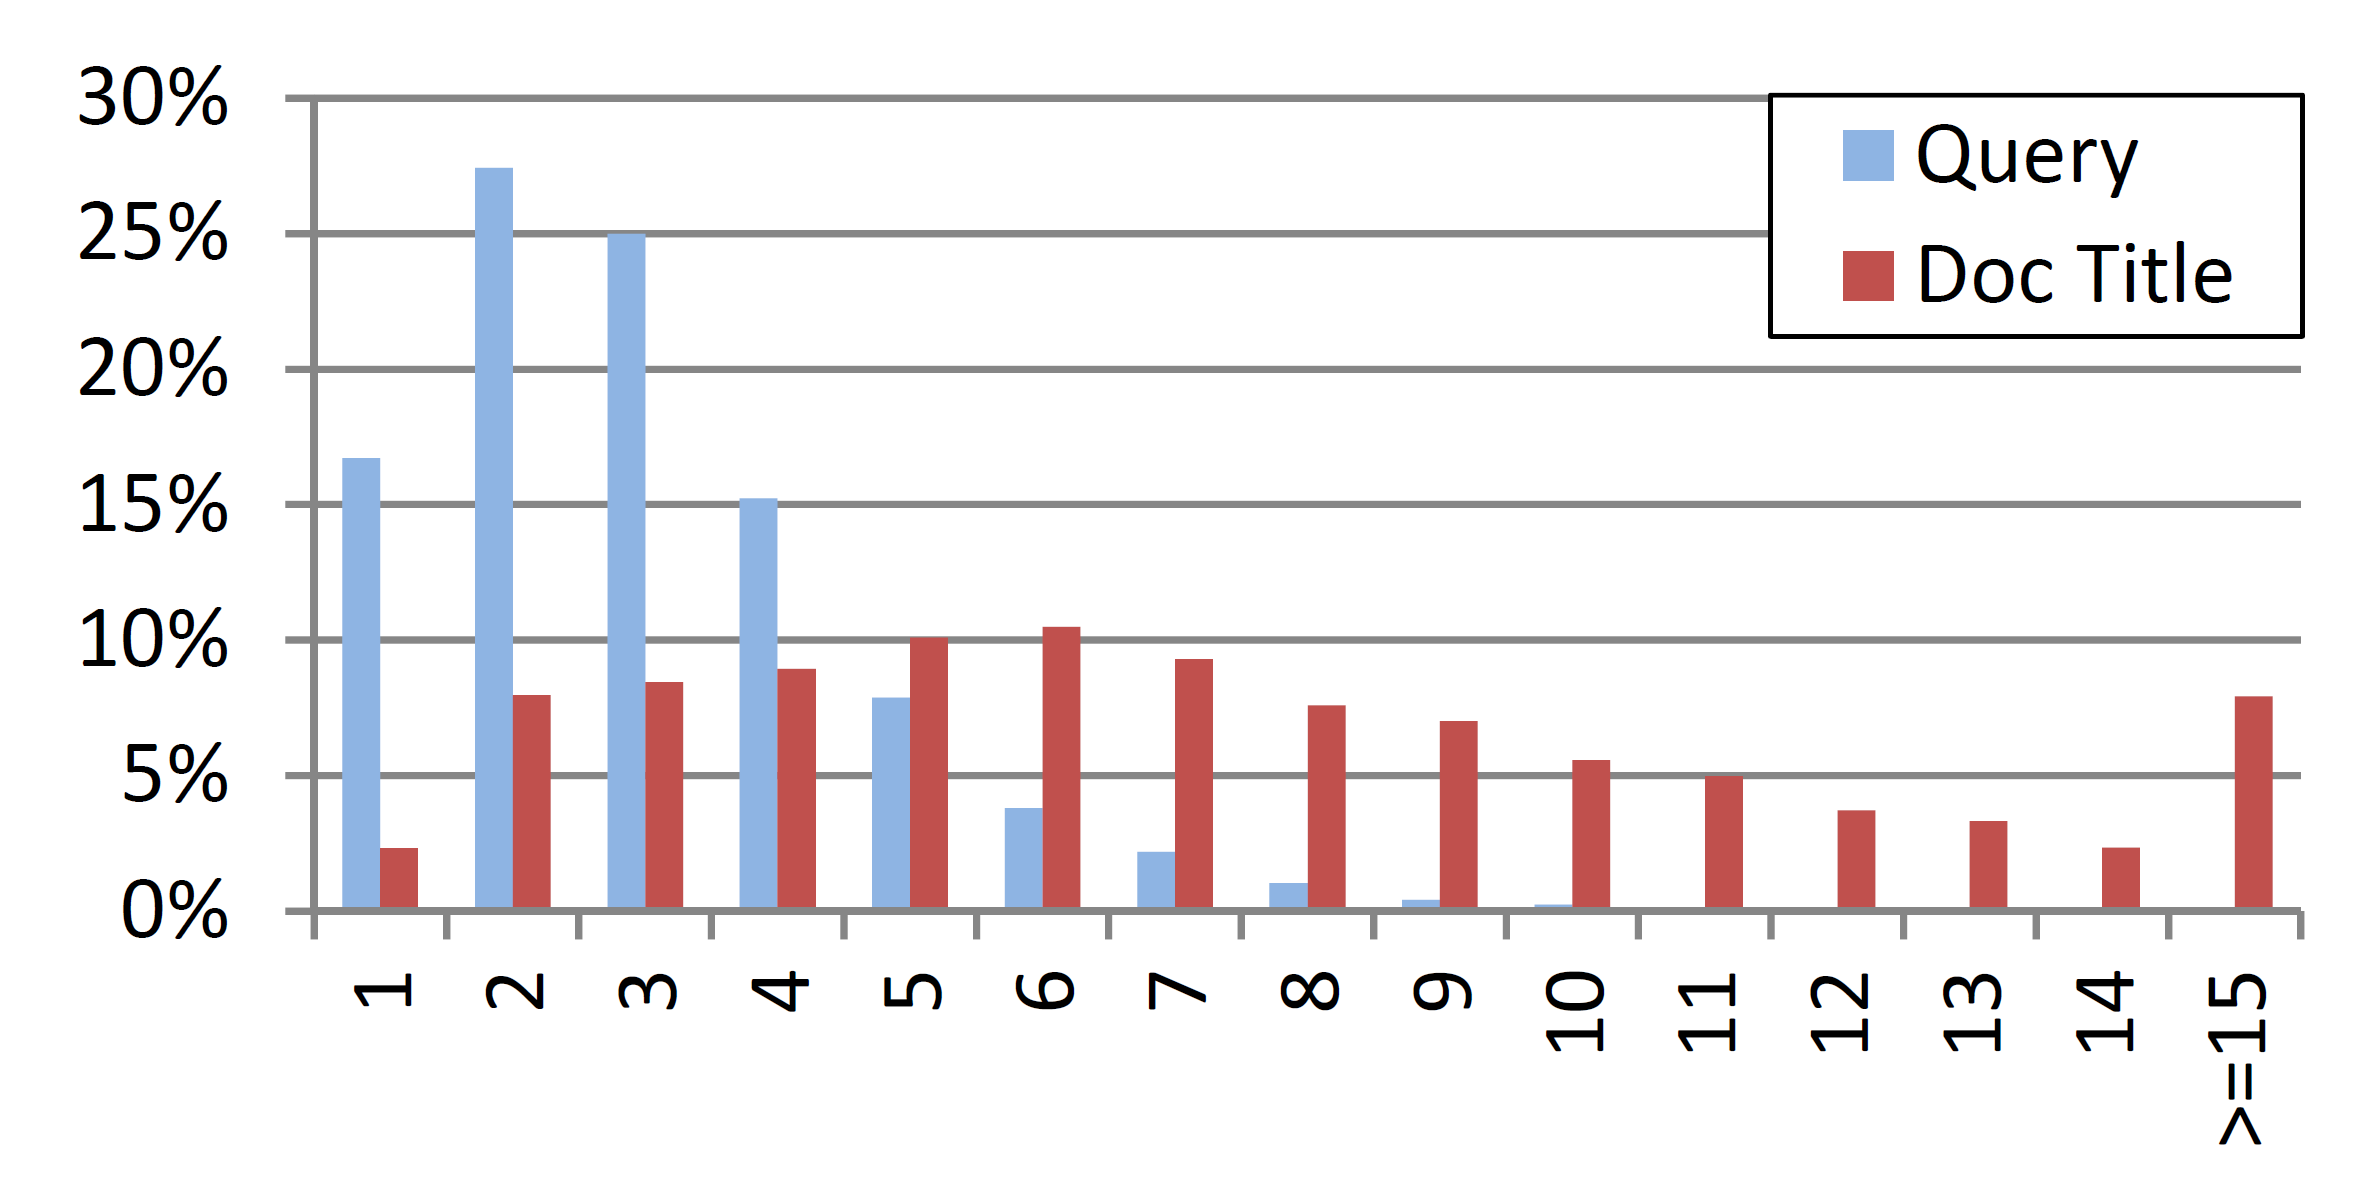
\includegraphics[width = \textwidth]{./Distribution.png}\\
%	\PlakatBildUnterschrift{\textbf{Figure 4:} Distribution of evalution data}	
%\end{figure}

\begin{table}[]
	\begin{tabular}{l|l|l|l|l}
		\#                                                & Models           & NDCG@1 & NDCG@3 & NDCG@10 \\
		\hline
		1                                                 & BM25             & 0.305  & 0.328  & 0.388   \\
		2                                                 & ULM              & 0.304  & 0.327  & 0.385   \\
		$\cdot$ &                  &        &        &         \\
		$\cdot$ &                  &        &        &         \\
		$\cdot$ &                  &        &        &         \\
		11                                                & PTM (maxlen = 3) & $0.319^\alpha$  & $0.347^\alpha$  & $0.413^\alpha$   \\
		12                                                & DSSM (J = 4)     & $0.320^{\alpha}$ & $0.355^{\alpha}$  & $0.431^{\alpha}$   \\
		13                                                & DSSM (J = 50)    & $0.327^{\alpha \beta}$  & $0.355^{\alpha \beta}$  & $0.431^{\alpha \beta}$   \\
		14                                                & CLSM (J = 4)     & $0.342^{\alpha \beta \gamma}$  & $0.374^{\alpha \beta \gamma}$  & $0.447^{\alpha \beta \gamma}$   \\
		\textbf{15}                                                & \textbf{CLSM (J = 50)}    & $\mathbf{0.348^{\alpha \beta \gamma}}$  & $\mathbf{0.379^{\alpha \beta \gamma}}$  & $\mathbf{0.449^{\alpha \beta \gamma}}$  
	\end{tabular}
	\vspace{5mm}
	\PlakatBildUnterschrift{\textbf{Table 1:} Comparison between state-of-the-art approaches. Superscripts $\alpha$,$\beta$, and $\gamma$ indicate statistically significant improvements over \textbf{BM25, PTM,} and \textbf{DSSM (J = 50)}, respectively.}
\end{table}

\begin{itemize}
	\item DSSM and CLSM are closely related in terms of the architecture and it is therefore feasible to compare them closer:
\end{itemize}

\begin{figure}
	
	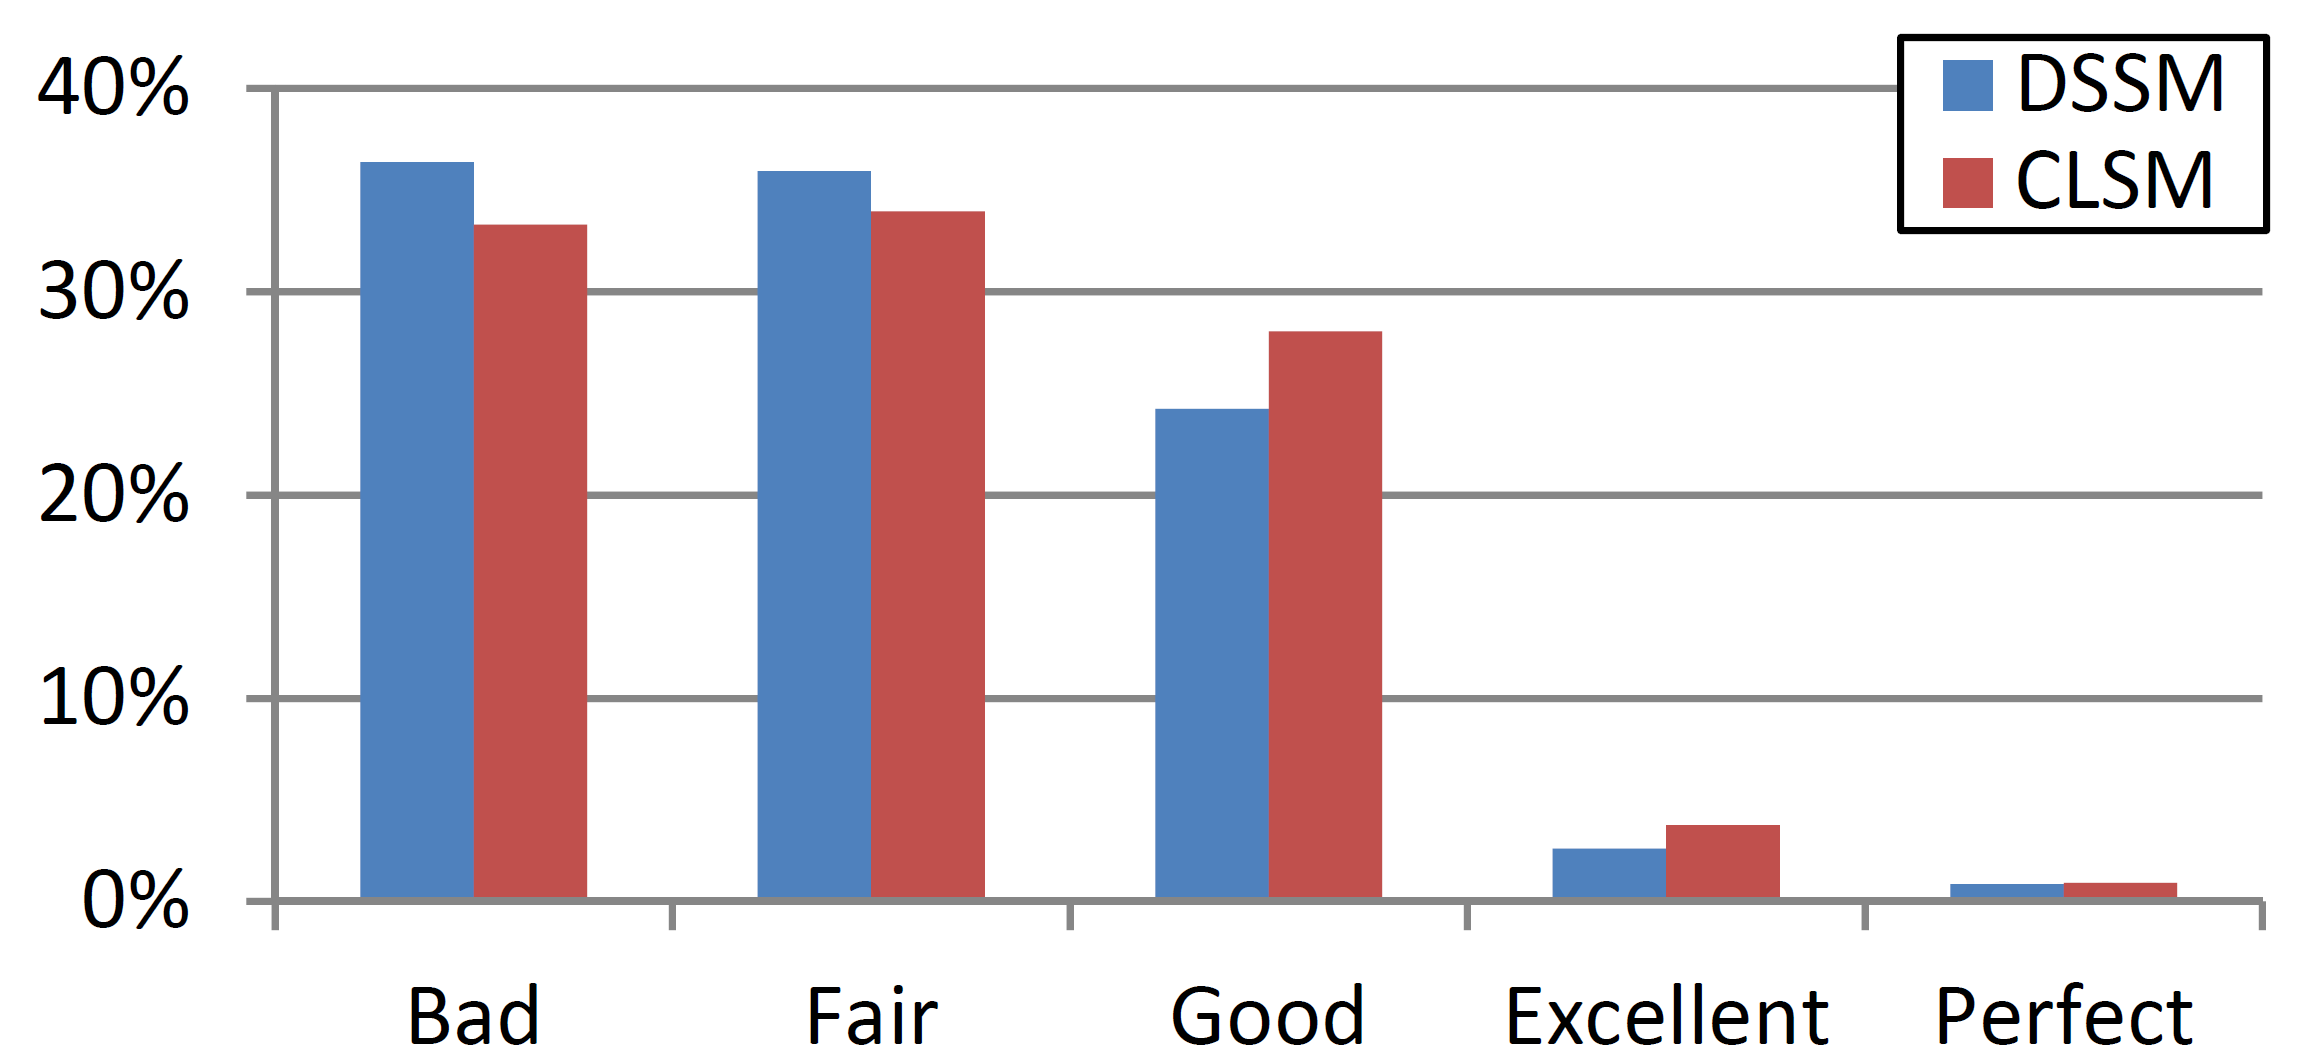
\includegraphics[width = \textwidth]{./Distribution2.png}\\
	\PlakatBildUnterschrift{\textbf{Figure 4:} Comparison of DSSM \footnote{\label{foot:1} Deep Structured Semantic Model} and CLSM regarding qualification quality}
	
\end{figure}

\vspace{20mm}

%\begin{figure}
	
%	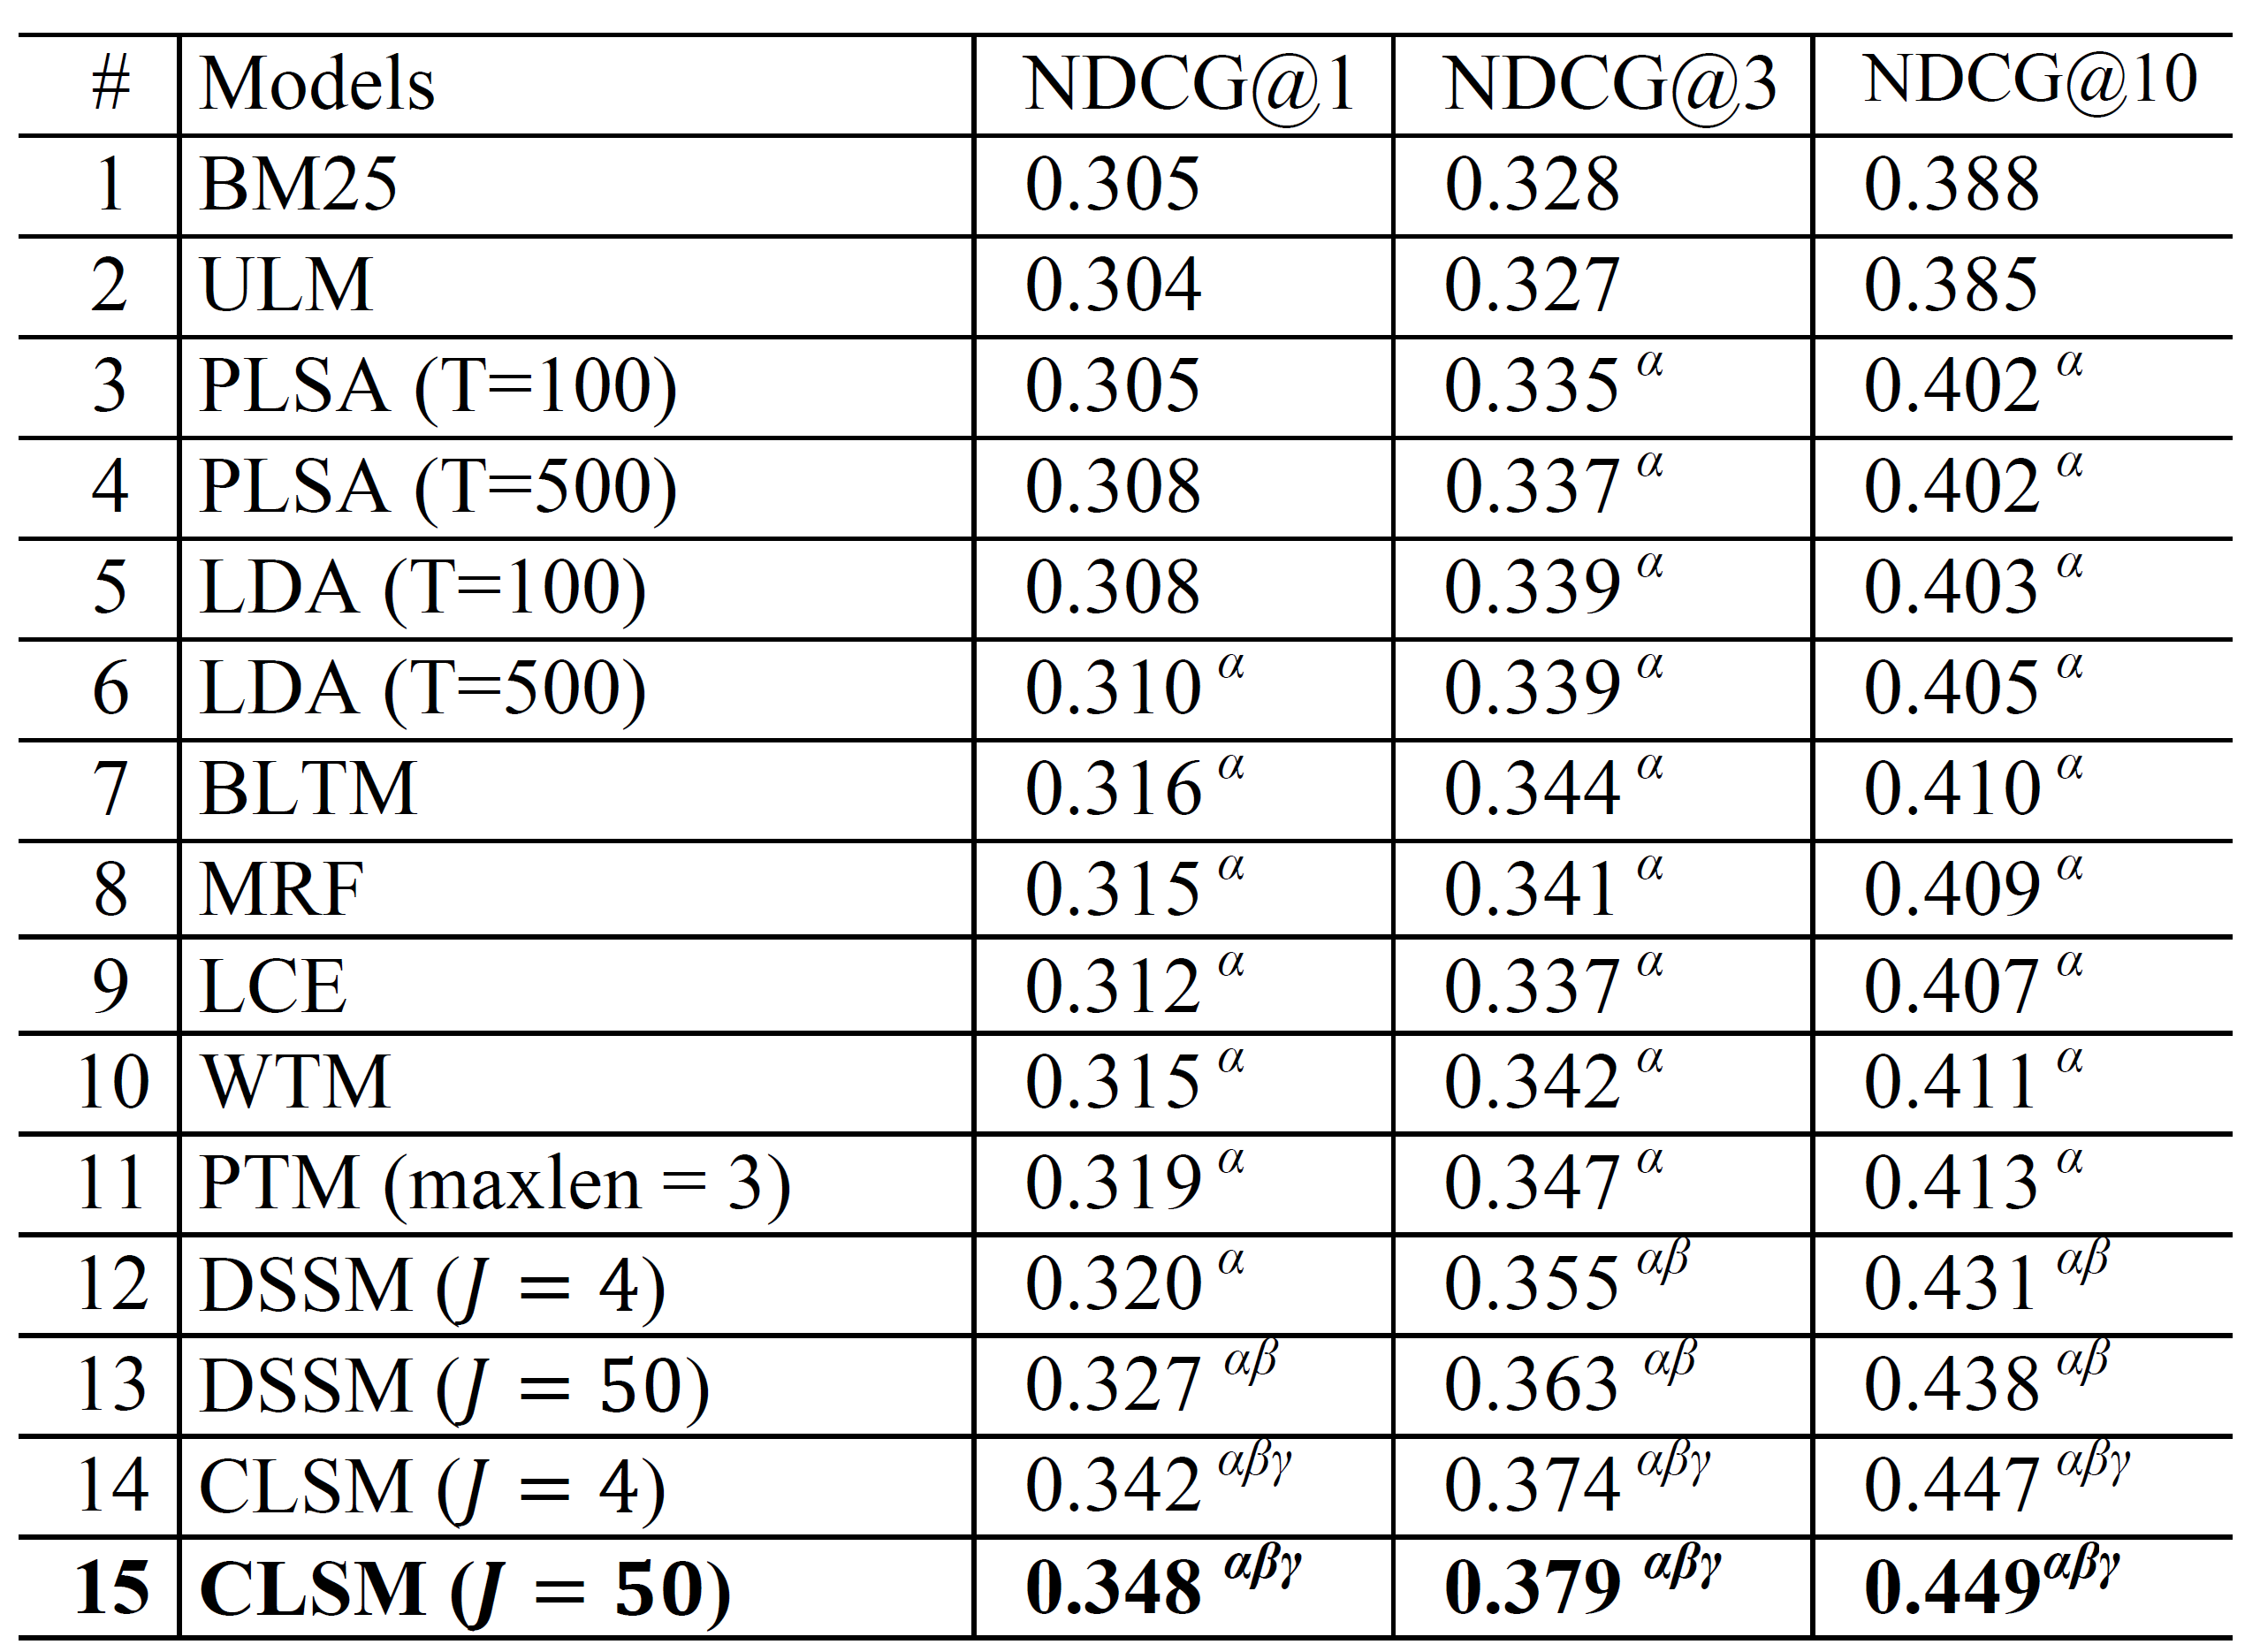
\includegraphics[width = \textwidth]{./table.png}\\
%	\PlakatBildUnterschrift{\textbf{Table 1:} Comparison between state-of-the-art approaches}
	
%\end{figure}


\end{multicols*}

\clearpage



%%%%%%%%%%%%%%%%%%%%%%%%%%%%%%%%%%%%%%%%%%%%%%%%%%%%%%%%%%%%%%%%%%%%%%%%%%%%%%%%
\end{document} % !!! NICHT ENTFERNEN !!!
%%%%%%%%%%%%%%%%%%%%%%%%%%%%%%%%%%%%%%%%%%%%%%%%%%%%%%%%%%%%%%%%%%%%%%%%%%%%%%%%
